%
% position5-small.tex
%
% (c) 2021 Prof Dr Andreas Müller, OST Ostschweizer Fachhochschule
%
\documentclass[tikz]{standalone}
\usepackage{times}
\usepackage{amsmath}
\usepackage{txfonts}
\usepackage[utf8]{inputenc}
\usepackage{graphics}
\usetikzlibrary{arrows,intersections,math}
\usepackage{ifthen}
\begin{document}

%
% common.tex
%
% (c) 2022 Prof Dr Andreas Müller, OST Ostschweizer Fachhochschule
%

\def\labelA{\node at (0.7,3.8) {$A$};}
\def\labelB{\node at (-3.4,-0.8) {$B$};}
\def\labelC{\node at (3.3,-2.1) {$C$};}
\def\labelP{\node at (-1.4,-3.5) {$P$};}

\def\labelc{\node at (-1.9,2.1) {$c$};}
\def\labela{\node at (-0.2,-1.2) {$a$};}
\def\labelb{\node at (2.6,1.5) {$b$};}

\def\labelhb{\node at (-2.6,-2.2) {$p_B$};}
\def\labelhc{\node at (1,-2.9) {$p_C$};}
\def\labell{\node at (-0.7,0.3) {$l$};}

\def\labelalpha{\node at (0.6,2.85) {$\alpha$};}
\def\labelbeta{\node at (-2.5,-0.5) {$\beta$};}
\def\labelgamma{\node at (2.3,-1.2) {$\gamma$};}
\def\labelomega{\node at (0.85,3.3) {$\omega$};}

\def\labelgammaone{\node at (2.1,-2.0) {$\gamma_1$};}
\def\labelgammatwo{\node at (2.3,-1.3) {$\gamma_2$};}
\def\labelbetaone{\node at (-2.4,-1.4) {$\beta_1$};}
\def\labelbetatwo{\node at (-2.5,-0.8) {$\beta_2$};}

\def\labelomegalinks{\node at (0.25,3.25) {$\omega$};}
\def\labelomegarechts{\node at (0.85,3.1) {$\omega$};}



\newboolean{showgrid}
\setboolean{showgrid}{false}
\def\breite{4}
\def\hoehe{4}

\begin{tikzpicture}[>=latex,thick,scale=0.625]

% Povray Bild
\node at (0,0) {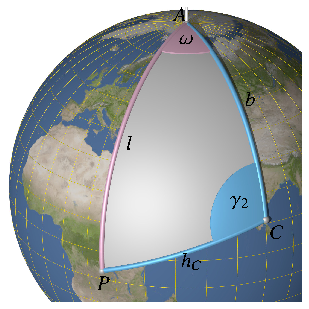
\includegraphics[width=5cm]{position5.jpg}};

% Gitter
\ifthenelse{\boolean{showgrid}}{
\draw[step=0.1,line width=0.1pt] (-\breite,-\hoehe) grid (\breite, \hoehe);
\draw[step=0.5,line width=0.4pt] (-\breite,-\hoehe) grid (\breite, \hoehe);
\draw                            (-\breite,-\hoehe) grid (\breite, \hoehe);
\fill (0,0) circle[radius=0.05];
}{}

\labelA
\labelC
\labelP

\labelb
\labell
\labelhc

\labelomegarechts
\labelgammatwo

\end{tikzpicture}

\end{document}

